\section{Models Used}
% Delete the text and write your Method(s) here:
%------------------------------------
\begin{figure}
    \centering
    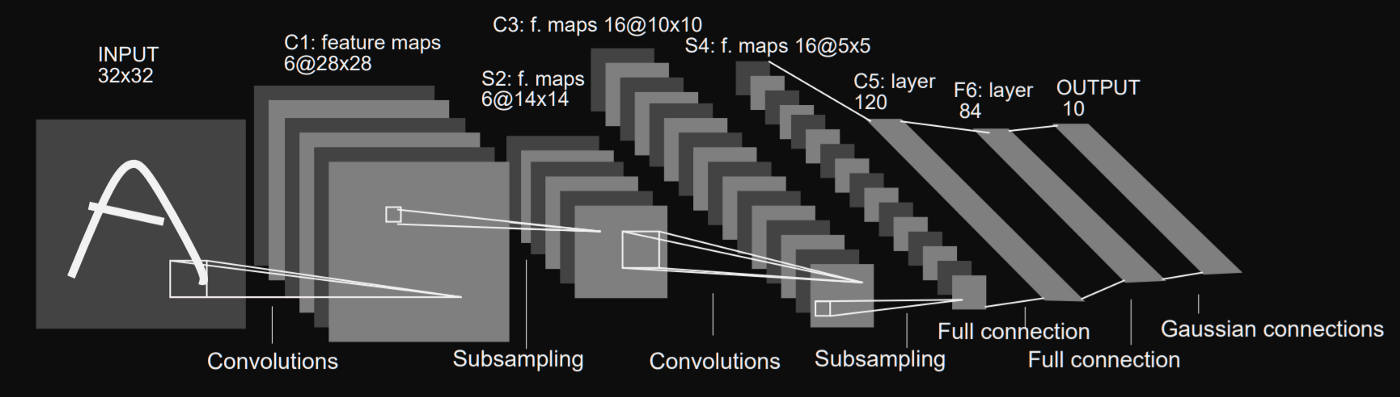
\includegraphics[width=0.48\textwidth]{Images/lenet_arcj.png}
    \caption{LeNet-5 Architecture}
    \label{fig:lenet-arch}
\end{figure}
\begin{figure}
    \centering
    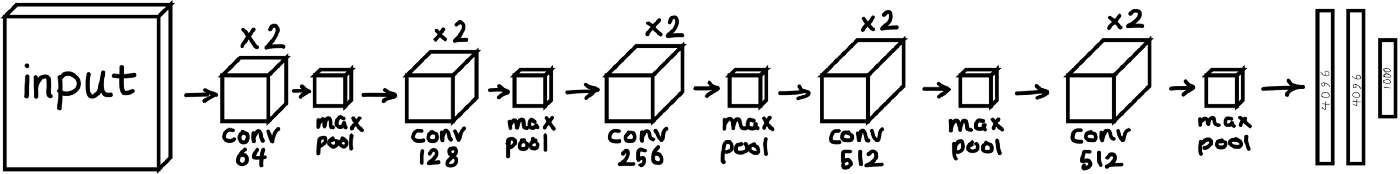
\includegraphics[width=0.48\textwidth]{Images/vgg-13-diag.png}
    \caption{Flow Diagram for VGG-13 Architecture}
    \label{fig:vgg-13-diag}
\end{figure}
\begin{figure}
    \centering
    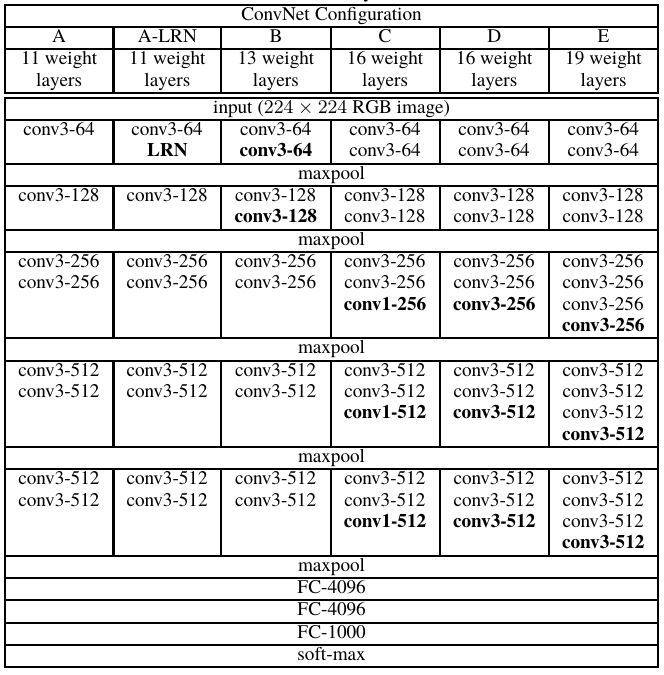
\includegraphics[width=0.48\textwidth]{Images/vgg_list.png}
    \caption{List Of VGG Architectures.}
    \label{fig:vgg-list}
\end{figure}
\subsection{VGG}
VGG stands for Visual Geometry Group; it is a standard deep Convolutional Neural Network (CNN) architecture with multiple layers. The “deep” refers to the number of layers with VGG-16 or VGG-19 consisting of 16 and 19 convolutional layers.\par

The VGG architecture is the basis of ground-breaking object recognition models. Developed as a deep neural network, the VGGNet also surpasses baselines on many tasks and datasets beyond ImageNet. Moreover, it is now still one of the most popular image recognition architectures.\par

This study uses VGG-3 and VGG-13 as the two different machine learning networks.\par 
To make the study simple, VGG-13 was chosen as it is the easier to implement out of multi layered machine learning networks. Following the same logic VGG-16 and VGG-19 can also be easily implemented for the dataset. \cref{fig:vgg-list} describes VGG-13 and others in a table. \par
VGG13 is model B in  \cref{fig:vgg-list}. A diagram can be found in \cref{fig:vgg-13-diag} to simplify how VGG-13 works in back.
\subsection{LeNet}

LeNet was introduced in the research paper “Gradient-Based Learning Applied To Document Recognition” in the year 1998 by Yann LeCun, Leon Bottou, Yoshua Bengio, and Patrick Haffner. Many of the listed authors of the paper have gone on to provide several significant academic contributions to the field of deep learning.\par
LeNet-5 CNN architecture is made up of 7 layers. The layer composition consists of 3 convolutional layers, 2 subsampling layers and 2 fully connected layers. \par

\cref{fig:lenet-arch} shows a depiction of the LeNet-5 architecture, as illustrated in the original paper. \par

The LeNet architecture is an excellent “first architecture” for Convolutional Neural Networks. LeNet is small and easy to understand — yet large enough to provide interesting results. Furthermore, the combination of LeNet + MNIST is able to run on the CPU, making it easy for beginners to take their first step in Deep Learning and Convolutional Neural Networks. \par

\subsection{CNN}
A convolutional neural network (CNN) is a type of artificial neural network used in image recognition and processing that is specifically designed to process pixel data.\par

CNNs are powerful image processing, artificial intelligence (AI) that use deep learning to perform both generative and descriptive tasks, often using machine vison that includes image and video recognition, along with recommender systems and natural language processing (NLP).\par

A neural network is a system of hardware and/or software patterned after the operation of neurons in the human brain. Traditional neural networks are not ideal for image processing and must be fed images in reduced-resolution pieces. CNN have their “neurons” arranged more like those of the frontal lobe, the area responsible for processing visual stimuli in humans and other animals. The layers of neurons are arranged in such a way as to cover the entire visual field avoiding the piecemeal image processing problem of traditional neural networks.\par

 \subsection{k-Fold Cross Validation}
 Cross-validation is a resampling procedure used to evaluate machine learning models on a limited data sample. \par

The procedure has a single parameter called k that refers to the number of groups that a given data sample is to be split into. As such, the procedure is often called k-fold cross-validation. When a specific value for k is chosen, it may be used in place of k in the reference to the model, such as k=10 becoming 10-fold cross-validation.\par

Cross-validation is primarily used in applied machine learning to estimate the skill of a machine learning model on unseen data. That is, to use a limited sample in order to estimate how the model is expected to perform in general when used to make predictions on data not used during the training of the model.\par
\begin{figure}
    \centering
    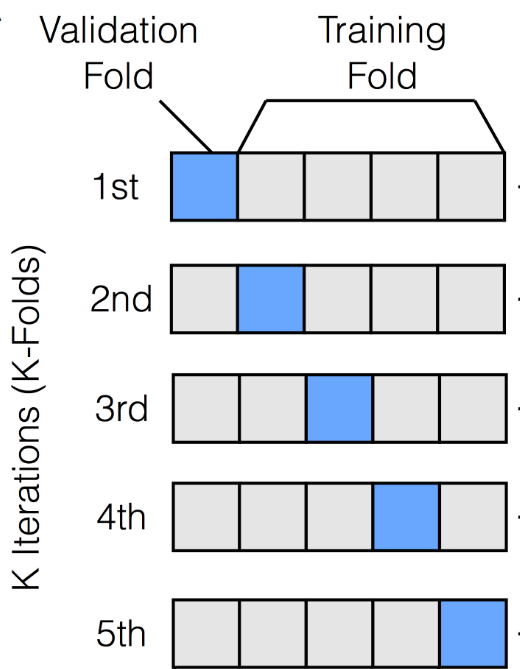
\includegraphics[width=0.48\textwidth]{Images/cross_validation.png}
    \caption{5-Fold Cross Validation Visualization}
    \label{fig:cross_validation}
\end{figure}
For cross validation kfold method from sklearn library is used. KFold method automatizises the cross validation that we do in our models' training. Figure  \cref{fig:cross_validation} represents how our 5 fold cross validation works in action. \par
How the K-Fold Cross validation is implemented is discussed in Appendix section of this paper.\par
